% Figure from MATH 493 notes, section 55 (the group Z/7Z x| Z/3Z as a grid). Added, not from lecture.
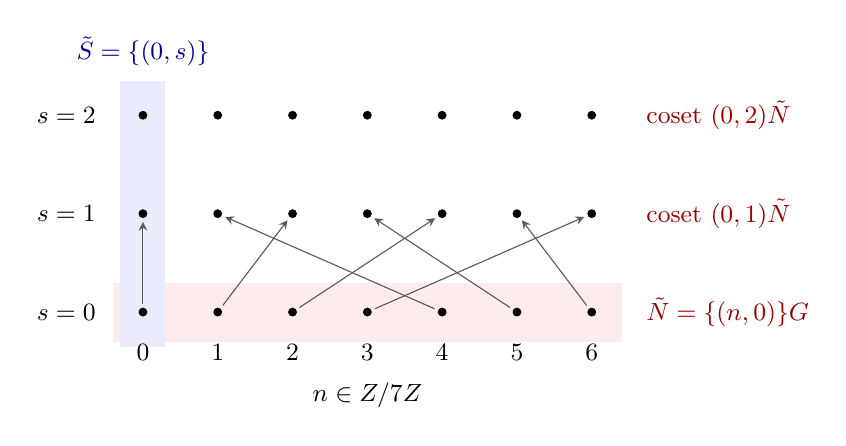
\begin{tikzpicture}[>=stealth, font=\small, x=0.95cm, y=1.25cm]
    \fill[red!8] (-0.4,-0.3) rectangle (6.4,0.3); \fill[blue!8] (-0.3,-0.35) rectangle (0.3,2.35);
    \fill (0,0) circle (1.6pt);
    \fill (1,0) circle (1.6pt);
    \fill (2,0) circle (1.6pt);
    \fill (3,0) circle (1.6pt);
    \fill (4,0) circle (1.6pt);
    \fill (5,0) circle (1.6pt);
    \fill (6,0) circle (1.6pt);
    \node[anchor=east] at (-0.5,0) {$s = 0$};
    \fill (0,1) circle (1.6pt);
    \fill (1,1) circle (1.6pt);
    \fill (2,1) circle (1.6pt);
    \fill (3,1) circle (1.6pt);
    \fill (4,1) circle (1.6pt);
    \fill (5,1) circle (1.6pt);
    \fill (6,1) circle (1.6pt);
    \node[anchor=east] at (-0.5,1) {$s = 1$};
    \fill (0,2) circle (1.6pt);
    \fill (1,2) circle (1.6pt);
    \fill (2,2) circle (1.6pt);
    \fill (3,2) circle (1.6pt);
    \fill (4,2) circle (1.6pt);
    \fill (5,2) circle (1.6pt);
    \fill (6,2) circle (1.6pt);
    \node[anchor=east] at (-0.5,2) {$s = 2$};
    \node[below=3pt] at (0,-0.15) {$0$};
    \node[below=3pt] at (1,-0.15) {$1$};
    \node[below=3pt] at (2,-0.15) {$2$};
    \node[below=3pt] at (3,-0.15) {$3$};
    \node[below=3pt] at (4,-0.15) {$4$};
    \node[below=3pt] at (5,-0.15) {$5$};
    \node[below=3pt] at (6,-0.15) {$6$};
    \draw[->, gray!70!black, shorten >=3pt, shorten <=3pt] (0,0) -- (0,1);
    \draw[->, gray!70!black, shorten >=3pt, shorten <=3pt] (1,0) -- (2,1);
    \draw[->, gray!70!black, shorten >=3pt, shorten <=3pt] (2,0) -- (4,1);
    \draw[->, gray!70!black, shorten >=3pt, shorten <=3pt] (3,0) -- (6,1);
    \draw[->, gray!70!black, shorten >=3pt, shorten <=3pt] (4,0) -- (1,1);
    \draw[->, gray!70!black, shorten >=3pt, shorten <=3pt] (5,0) -- (3,1);
    \draw[->, gray!70!black, shorten >=3pt, shorten <=3pt] (6,0) -- (5,1);
    \node[red!60!black, anchor=west] at (6.6,0) {$\tilde N = \{(n, 0)\} \trianglelefteq G$};
    \node[red!60!black, anchor=west] at (6.6,1) {coset $(0,1)\tilde N$};
    \node[red!60!black, anchor=west] at (6.6,2) {coset $(0,2)\tilde N$};
    \node[blue!60!black, anchor=south] at (0,2.4) {$\tilde S = \{(0, s)\}$};
    \node at (3,-0.85) {$n \in \mathbb{Z}/7\mathbb{Z}$};
\end{tikzpicture}
